\chapter{Model Evaluation and Results Analysis}
\label{chap:Chapter4}

This chapter provides an in-depth analysis of the performance and results obtained from testing the models in two distinct environments: the local testing environment and the live testing environment.

\section{Local Testing Environment}

In the local testing environment, the models were evaluated using a dataset that was split into training and testing subsets

Due to hardware limitations\footnote{Training a single alert takes 10 to 15 minutes, making it impractical to train on 100k alerts in a reasonable timeframe.}, the RL model was not tested on this environment, therefore, the results presented in this section are only of the RF model's performance and its evolution from Version 1 to Version 11.

The RF model was trained and tested on the dataset, and its performance was measured using metrics such as accuracy, precision, recall, and F1-score.
\begin{itemize}
    \item \textbf{Accuracy:} The proportion of correctly classified alerts out of the total alerts.
    \item \textbf{Precision:} The ratio of true positive predictions to the total predicted positives, indicating the model's ability to avoid false positives.
    \item \textbf{Recall:} The ratio of true positive predictions to the total actual positives, reflecting the model's ability to capture all relevant alerts.
    \item \textbf{F1-score:} The harmonic mean of precision and recall, providing a balanced measure of the model's performance.
\end{itemize}

The values for all the metrics are based on the final results from training. 
Since, after training the model, that same model is tested against a test data subset, it is possible to get values for the model's performance and accuracy.

Table~\ref{tab:results_comparative} shows the values for the metrics of Version 1 and Version 11, showing the evolution of the model from the first to the last version.

\clearpage

\begin{table}[h!]
    \centering
    \begin{tabular}{@{}ccccc@{}}
        \toprule
        \multirow{2}{0em}{} & \multicolumn{2}{c}{\textbf{Priority}} & \multicolumn{2}{c}{\textbf{Taxonomy}} \\
        & \textbf{Version 1} & \textbf{Version 11} & \textbf{Version 1} & \textbf{Version 11} \\
        \hline
        \textbf{Accuracy} & 82\% & 90\% & 82\% & 90\% \\
        \textbf{Precision} & 82\% & 89\% & 81\% & 90\% \\
        \textbf{Recall} & 80\% & 89\% & 65\% & 90\% \\
        \textbf{F1-Score} & 82\% & 89\% & 69\% & 90\% \\
        \bottomrule
    \end{tabular}
    \caption{Model Performance Metrics Comparison: Version 1 vs. Version 11}
    \label{tab:results_comparative}
\end{table}

From the table, it is evident that Version 11 demonstrates notable improvements over Version 1 in all metrics. Specifically:

\begin{itemize}
    \item \textbf{Accuracy:} Both priority and taxonomy classifications improved from 82\% in Version 1 to 90\% in Version 11, indicating a higher proportion of correctly classified alerts overall.
    \item \textbf{Precision:} The precision for priority classification increased from 82\% to 89\%, and for taxonomy classification, it rose from 81\% to 90\%. Making it clear that Version 11 is better at minimizing false positives.
    \item \textbf{Recall:} A significant improvement is observed in recall, particularly for priority classification, which increased from 65\% in Version 1 to 90\% in Version 11. This indicates that the model is now more effective at identifying true positives, especially for minority or low-frequency categories.
    \item \textbf{F1-Score:} The F1-Score, which balances precision and recall, also improved from 69\% to 90\% for priority classification, reflecting the overall enhancement in the model's robustness.
\end{itemize}

These improvements highlight the evolution of the model's ability to handle complex classification tasks, particularly in addressing challenges associated with low-frequency categories. 
The enhanced recall for minority classes is particularly noteworthy, as it demonstrates the model's capacity to reduce bias and improve fairness in predictions.

Besides accuracy, recall is a fundamental factor, as being able to correctly identify an alert for what it truly is—whether in terms of priority or taxonomy—is critical. 
Confusing a P1 (high priority) with a P3 (low priority) can have serious consequences, potentially leading to delayed responses or misallocated resources.

Therefor, analyzing the confusion matrixes is essential to understand the model's performance in detail.
The confusion matrixes provide a visual representation of the model's performance, allowing us to see how well the model classifies each category and where it tends to make mistakes.

Figures~\ref{fig:confusion_priority_v1} and \ref{fig:confusion_priority_v11} illustrate the evolution of the model's performance in priority classification from Version 1 to Version 11. 

\clearpage

\begin{figure}[t!]
    \centering
    \begin{minipage}{0.49\textwidth}
        \centering
        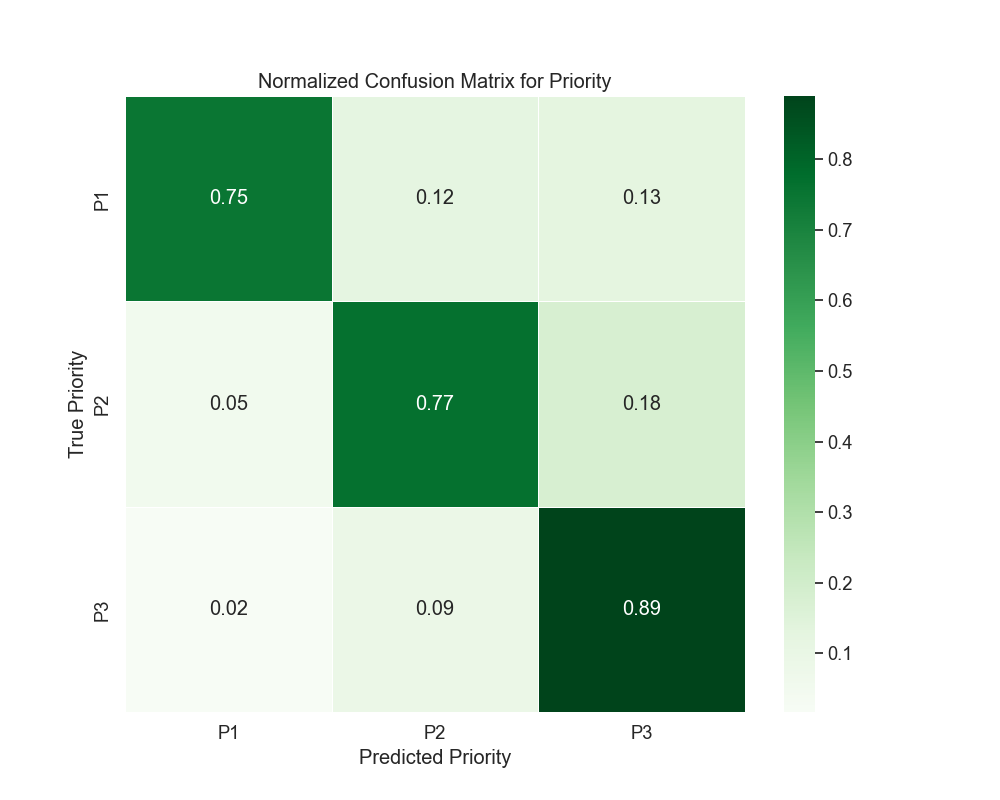
\includegraphics[width=\textwidth]{ch4/assets/v1_confusion_priority.png}
        \caption{Confusion Matrix for Priority (Version 1)}
        \label{fig:confusion_priority_v1}
    \end{minipage}
    \hfill
    \begin{minipage}{0.49\textwidth}
        \centering
        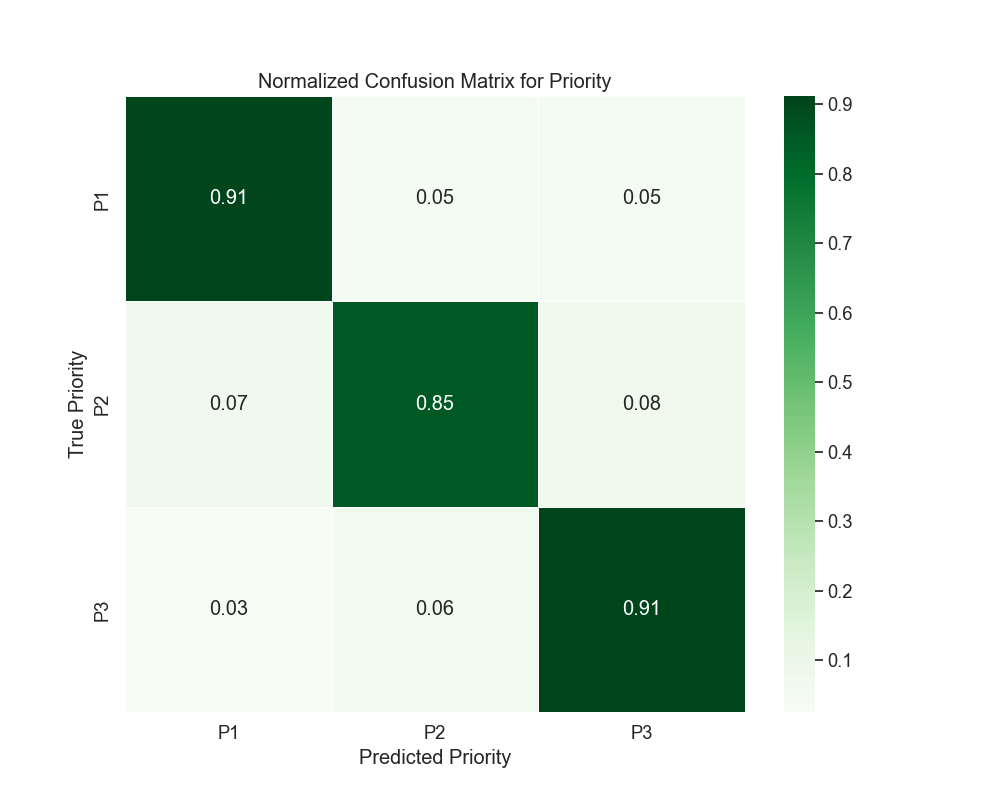
\includegraphics[width=\textwidth]{ch4/assets/v11_confusion_priority.png}
        \caption{Confusion Matrix for Priority (Version 11)}
        \label{fig:confusion_priority_v11}
    \end{minipage}
\end{figure}

In Version 1, the confusion matrix (Figure~\ref{fig:confusion_priority_v1}) reveals notable misclassifications, particularly between P1 and P2 categories. 
The recall values for P1 and P2 were 0.75 and 0.77, respectively, while P3 achieved a higher recall of 0.89, indicating relatively better performance for lower-priority classes. 

In contrast, Version 11 (Figure~\ref{fig:confusion_priority_v11}) demonstrates significant improvements, achieving recalls of 0.91 for P1, 0.85 for P2, and 0.91 for P3. 
These enhancements reflect a substantial reduction in misclassifications, particularly between P1 and P2, showcasing the model's improved ability to differentiate between priority levels. 

The key advancements from Version 1 to Version 11 are evident in the increased recall for P2, which rose from 0.77 to 0.85, and for P3, which improved from 0.89 to 0.91. 
These results underscore the model's enhanced accuracy and robustness in handling priority-based predictions, particularly for categories that were previously challenging to classify accurately.

The same analysis can be applied to taxonomy classification, where the confusion matrixes provide insights into the model's performance across different categories.

In Version 1 (Figure~\ref{fig:confusion_taxonomy_v1}), the model's performance was somewhat lacking, especially with low-frequency categories. 
For example:

\begin{itemize}
    \item \textbf{"Abusive Content"} had a recall of only \textbf{0.19}, meaning that a substantial portion of this class was misclassified.
    \item \textbf{"Fraud"} performed well with \textbf{0.95} recall, demonstrating that the model successfully identifies most instances of fraud.
    \item \textbf{"Vulnerable"} had \textbf{0.36} recall, indicating the model struggled to identify alerts related to vulnerabilities.
    \item \textbf{"Intrusions"} also performed poorly with \textbf{0.26} recall.
    \item \textbf{"Information Security"} was significantly more challenging with \textbf{0.03} recall, suggesting that the model could not detect a substantial portion of critical security threats in this category.
\end{itemize}

Whereas, in Version 11 (Figure~\ref{fig:confusion_taxonomy_v11}), the model's performance improved significantly across all categories.

In Version 11, several key improvements were made:

\begin{itemize}
    \item \textbf{"Abusive Content"} showed a dramatic improvement in recall to \textbf{0.46}, almost a threefold increase. The model is now better at identifying such content, which is crucial in detecting harmful communications or activity.
    \item \textbf{"Fraud"} maintained a high recall of \textbf{0.94}, demonstrating that the model continues to perform well in this critical category.
    \item \textbf{"Vulnerable"} showed a notable improvement in recall to \textbf{0.79}, addressing the initial weakness seen in Version 1. This is essential for detecting vulnerabilities and minimizing risks.
    \item \textbf{"Intrusions"} also improved significantly to \textbf{0.64}, indicating that the model is now better at identifying intrusion attempts, which are often targeted threats.
    \item \textbf{"Information Security"} improved from \textbf{0.03} in Version 1 to \textbf{0.32} in Version 11, reflecting a better capability to identify security-related alerts, which was a major challenge in the previous version.
\end{itemize}

\begin{figure}[h!]
    \centering
    \begin{minipage}{0.49\textwidth}
        \centering
        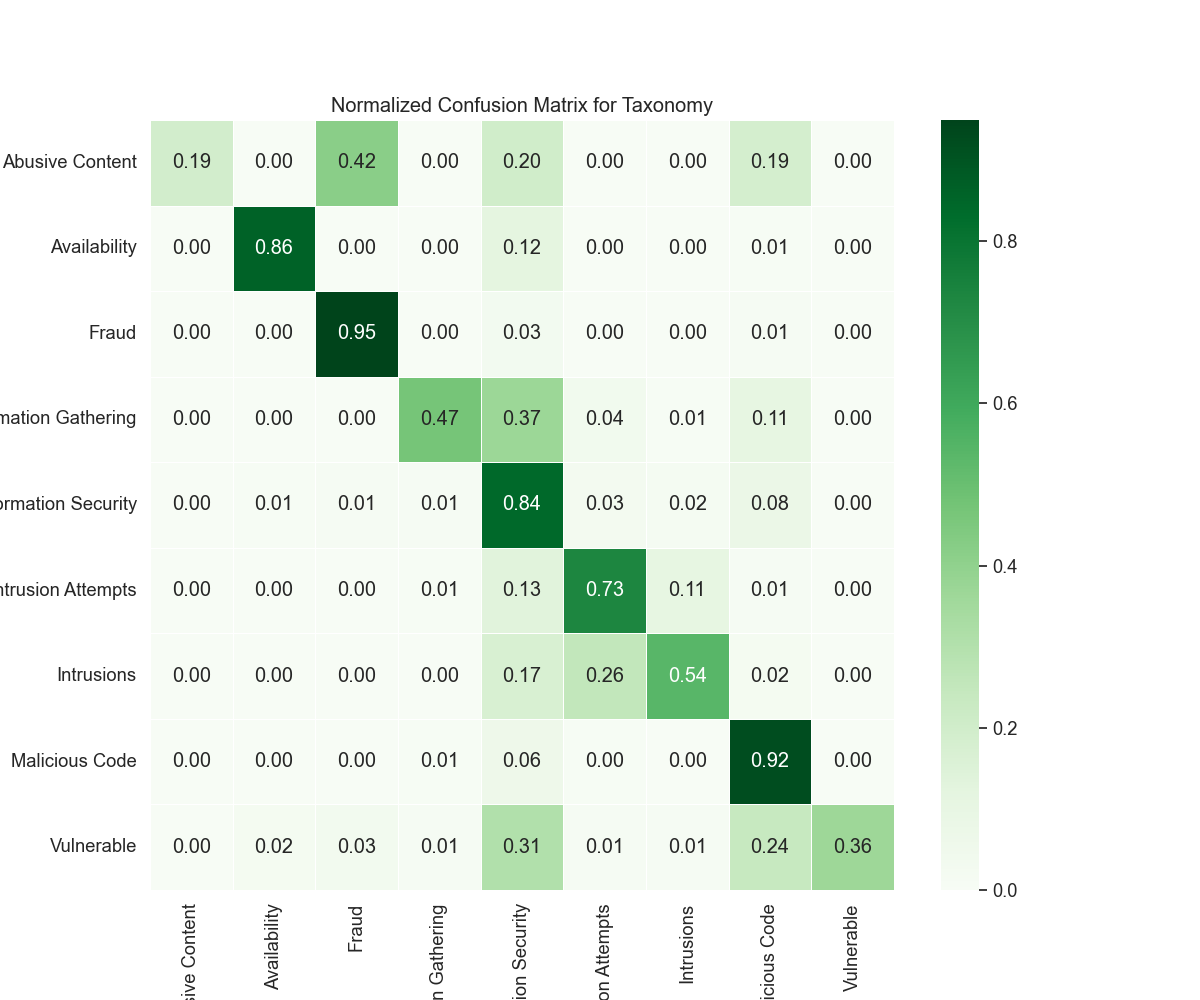
\includegraphics[width=\textwidth]{ch4/assets/v1_confusion_taxonomy.png}
        \caption{Confusion Matrix for Taxonomy (Version 1)}
        \label{fig:confusion_taxonomy_v1}
    \end{minipage}
    \hfill
    \begin{minipage}{0.49\textwidth}
        \centering
        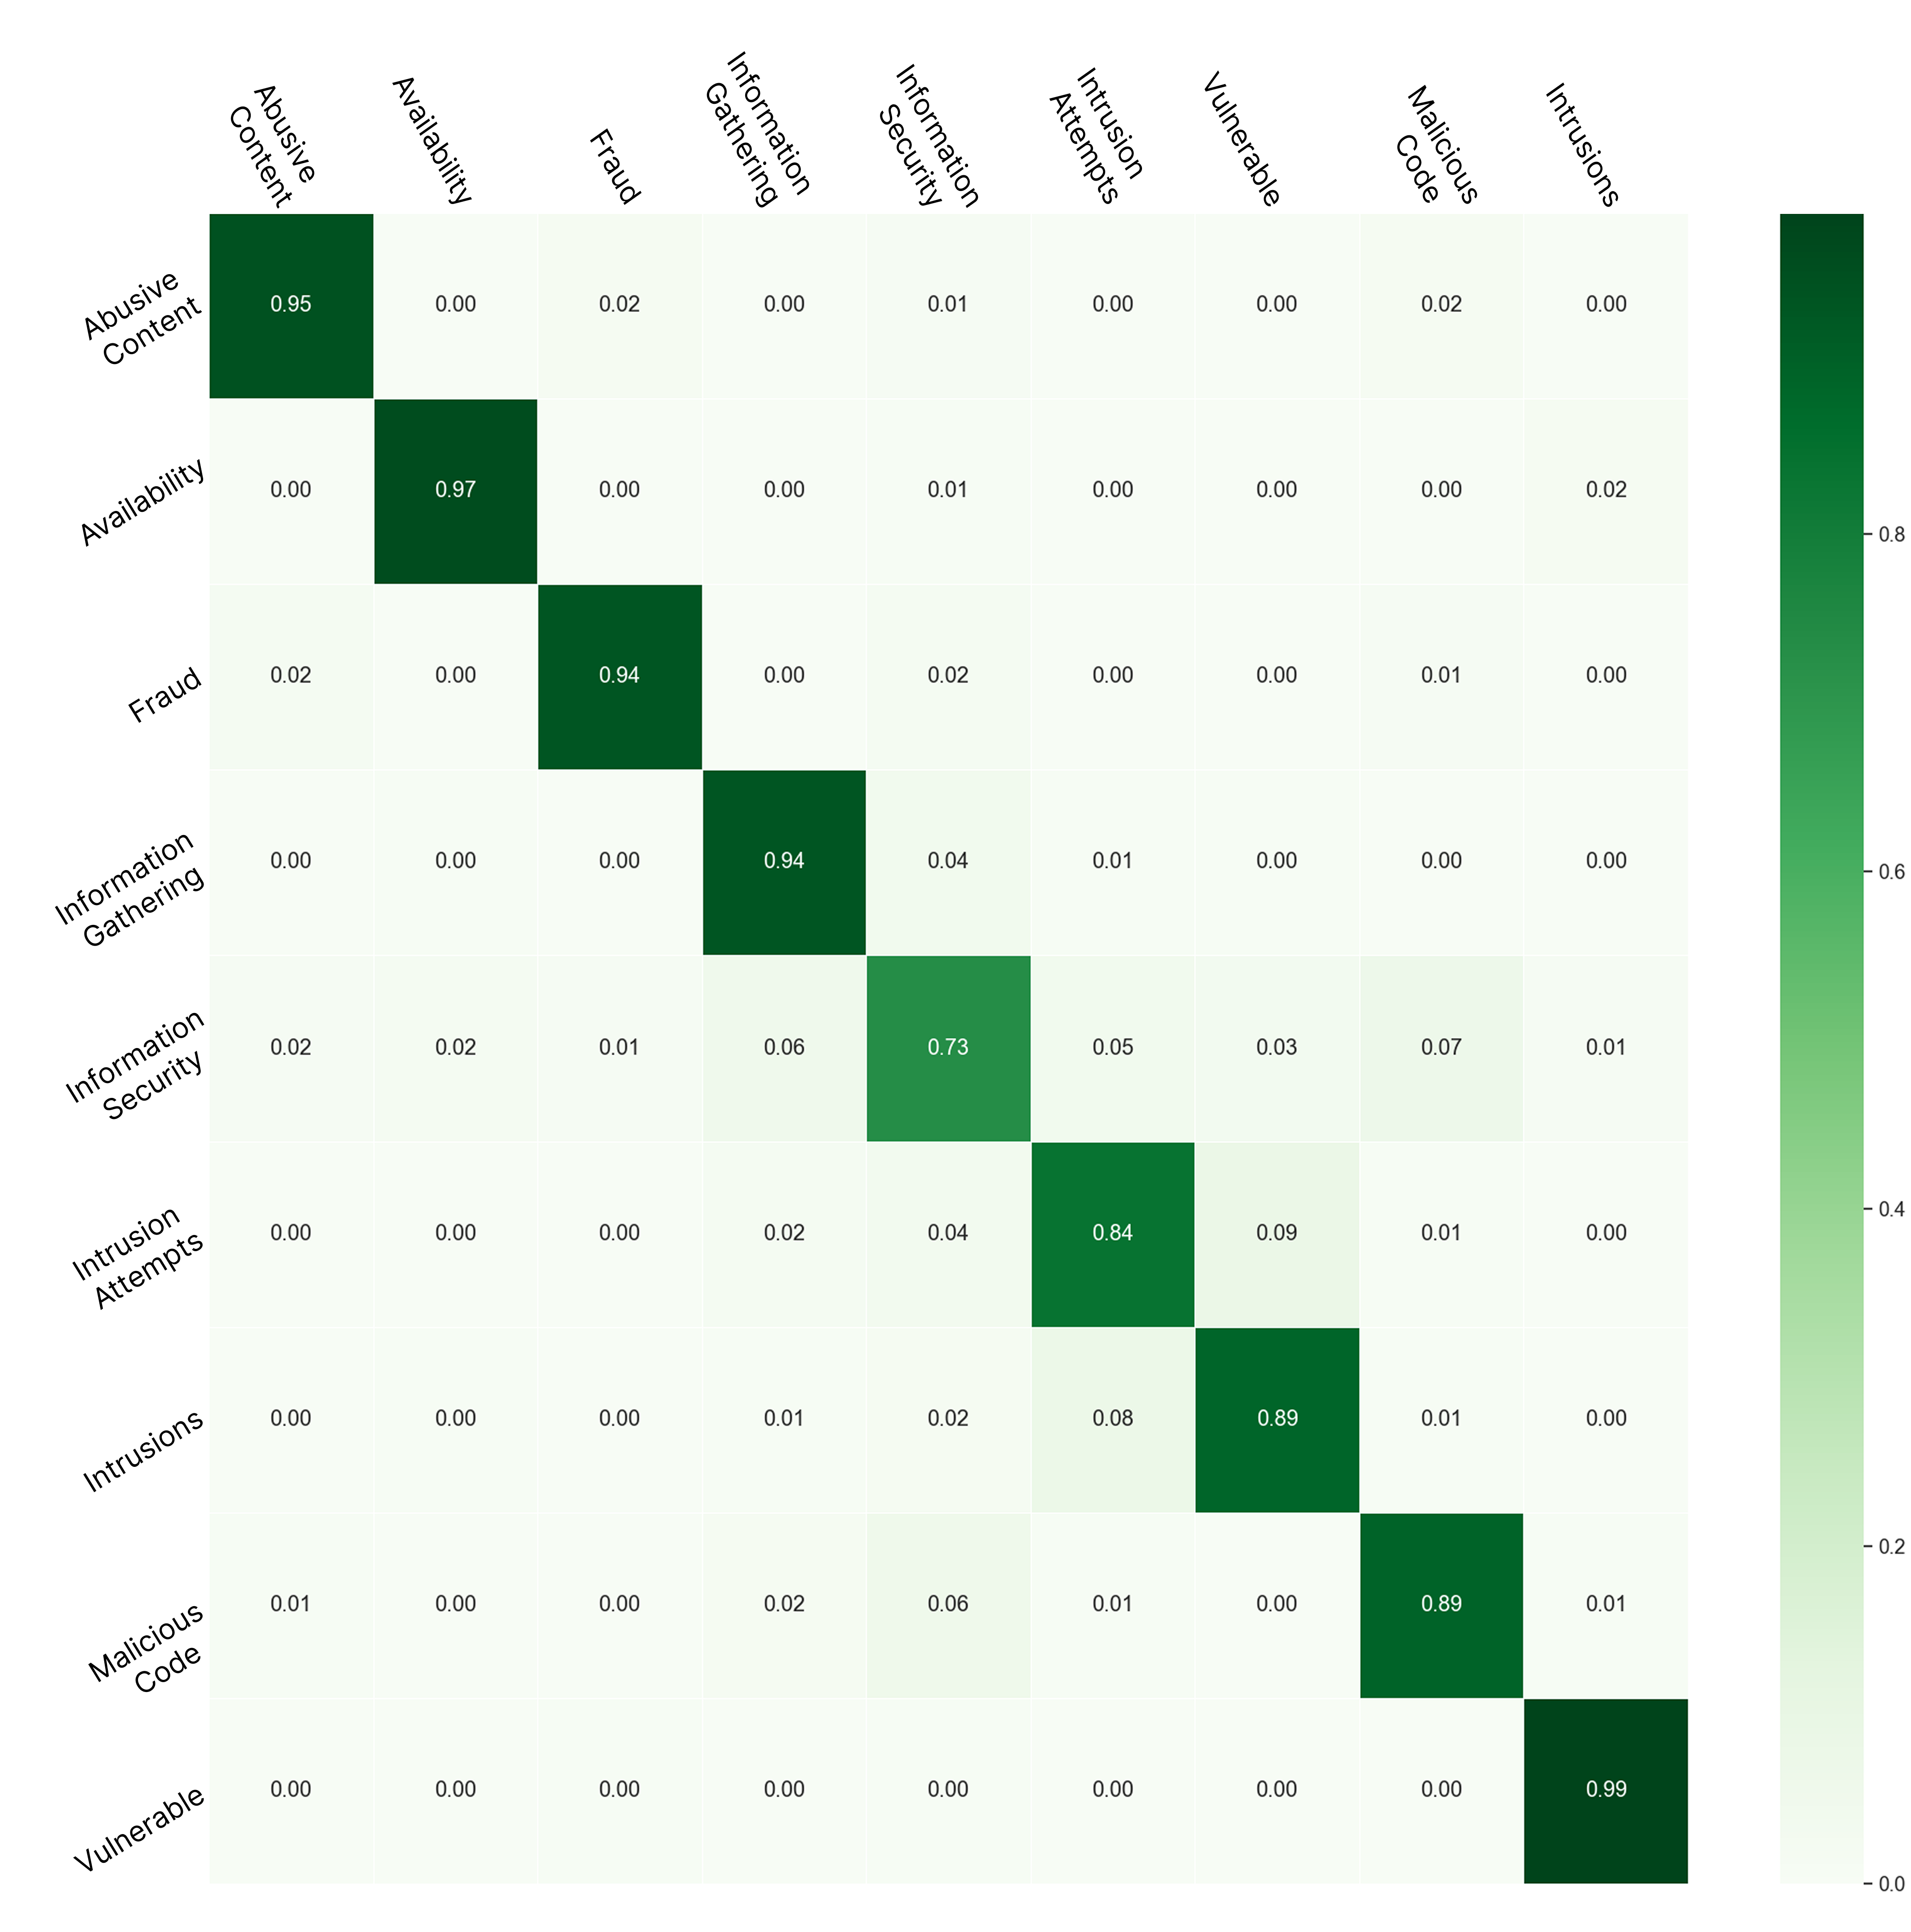
\includegraphics[width=\textwidth]{ch4/assets/v11_confusion_taxonomy.png}
        \caption{Confusion Matrix for Taxonomy (Version 11)}
        \label{fig:confusion_taxonomy_v11}
    \end{minipage}
\end{figure}

The improvements in recall across all categories in Version 11 indicate that the model is now more effective at identifying relevant alerts, particularly in low-frequency categories.
This is crucial for ensuring that the model can accurately classify and prioritize alerts, especially in cases where certain categories may have been previously overlooked or misclassified.

\section{Live Testing Environment}

The live testing environment aims to simulate real-world deployment, where the models are evaluated based on their actual performance in the company's infrastructure. 
In this environment, both the RF and RL models are expected to be used. 
However, unlike the local environment where testing was done solely on the RF model, the live environment will also involve continuous training of the RL model. 
As feedback is gathered, the RL model is expected to improve its performance over time.

For the live testing, the application will not be evaluated separately on the RF and RL models but will instead use both models as part of an integrated system. 
During this phase, feedback from real-time predictions will be used to adjust and fine-tune the RL model's decisions. 
The expectation is that with time, the RL model will show improvements in its ability to predict priority and taxonomy, surpassing the performance of the initial RF model version.
